%%% File encoding is ISO-8859-1 (also known as Latin-1)
%%% You can use special characters just like �,� and �
%%% LaTeX template by Manuel Kuehner, 2015

%%% If you use this template then please give credit like this:
%%% ----------------------------
% LaTeX code inspired by the LaTeX Thesis Template by Manuel Kuehner 
% www.bedienhaptik.de/latex-template/
%%% ----------------------------

% ##############################################
% Start: Template Preamble
% ##############################################
%

% Documentclass definition
%%% File encoding is ISO-8859-1 (also known as Latin-1)
%%% You can use special characters just like �,� and �

% KOMA-Script class 'scrbook'
% Link to the documentation: 
% German: http://mirrors.ctan.org/macros/latex/contrib/koma-script/doc/scrguide.pdf
% English: http://mirrors.ctan.org/macros/latex/contrib/koma-script/doc/scrguien.pdf
% CTAN: http://www.ctan.org/pkg/koma-script
% Author of the KOMA-Script family is Markus Kohm
\documentclass%
[%
paper=a4
,fontsize=12pt % common are 10, 11 or 12
,headings=big
,parskip
,numbers=noendperiod % 2.3.1 vs 2.3.1. (no dot after the last chapter number)
,twoside=true
,toc=bibliography % Bibliography appears in Table of Contents (without a number)
,toc=listof % List of Figures and List of Tables appear in Table of Contents
,version=last % Use latest version of the KOMA-Script
,openany
]%
{scrbook}

% Loading additional packages from the KOMA-Script family
%%% File encoding is ISO-8859-1 (also known as Latin-1)
%%% You can use special characters just like �,� and �

% Special KOMA-Script package - I added it because I also use the float package in this template, see: 
% http://tex.stackexchange.com/questions/51867/koma-warning-about-toc
% CTAN: http://www.ctan.org/tex-archive/macros/latex/contrib/koma-script/doc
\usepackage{scrhack}

% Better support for marginnotes
% new command: \marginnote
% LaTeX standard command: \marginpar
% CTAN: http://www.ctan.org/pkg/marginnote
\usepackage{marginnote}

% Extended header and footer support
% CTAN: http://www.ctan.org/pkg/scrpage2
\usepackage[%
  	automark
  	,ilines
	,headsepline
	,footsepline
]{scrlayer-scrpage}
% Page layout definition
%%% File encoding is ISO-8859-1 (also known as Latin-1)
%%% You can use special characters just like �,� and �

% User friendly interface to change layout parameters
% CTAN: http://www.ctan.org/pkg/geometry
\usepackage{geometry}
\geometry{% siehe geometry.pdf (Figure 1)
	bottom=30mm,
	showframe=false, % For debugging: try true and see the layout frames
	margin=30mm,
	marginparsep=3mm,
	marginparwidth=20mm
}

% Standard packages
%%% File encoding is ISO-8859-1 (also known as Latin-1)
%%% You can use special characters just like �,� and �

% Input encoding is 'latin1' (Latin 1 - also known as ISO-8859-1)
% CTAN: http://www.ctan.org/pkg/inputenc
% 
% A newer package is available - you may look into:
% \usepackage[x-iso-8859-1]{inputenc}
% CTAN: http://www.ctan.org/pkg/inputenx
\usepackage[latin1]{inputenc}

% Font Encoding is 'T1' -- important for special characters such as Umlaute � or � and special characters like � (enje)
% CTAN: http://www.ctan.org/pkg/fontenc
\usepackage[T1]{fontenc}

% Language support for 'english' (alternative 'ngerman' or 'french' for example)
% CTAN: http://www.ctan.org/pkg/babel
\usepackage[english]{babel} 

% Doing calculations with LaTeX units -- needed for the vertical line in the footer
% CTAN: http://www.ctan.org/pkg/calc
\usepackage{calc}

% Extended graphics support 
% There is also a package named 'graphics' - watch out!
% CTAN: http://www.ctan.org/pkg/graphicx
\usepackage{graphicx}

% Extendes support for floating objects (tables, figures), adds the [H] placing option (\begin{figure}[H]) which palces it "Here" (without any doubt).
% CTAN: http://www.ctan.org/pkg/float
\usepackage{float}

% Extended color support
% I use the command \definecolor for example. 
% Option 'Table': Load the colortbl package, in order to use the tools for coloring rows, columns, and cells within tables.
% CTAN: http://www.ctan.org/pkg/xcolor
\usepackage[table]{xcolor} 

% Nice tables
% CTAN: http://www.ctan.org/pkg/booktabs
\usepackage{booktabs}

% Better support for ragged left and right. Provides the commands \RaggedRight and \RaggedLeft. 
% Standard LaTeX commands are \raggedright and \raggedleft
% http://www.ctan.org/pkg/ragged2e
\usepackage{ragged2e}

% Create function plots directly in LaTeX
% CTAN: http://www.ctan.org/pkg/pgfplots
\usepackage{pgfplots}
\pgfplotsset{compat=1.11}

% Math stuff.
\usepackage{amsmath,amsfonts,amssymb}

% Code stuff.
\usepackage{listings}

\definecolor{mygreen}{rgb}{0,0.6,0}
\definecolor{mylightgray}{gray}{0.98}
\definecolor{mygray}{rgb}{0.5,0.5,0.5}
\definecolor{mymauve}{rgb}{0.58,0,0.82}
\lstset{ %
  backgroundcolor=\color{mylightgray},   % choose the background color; you must add \usepackage{color} or \usepackage{xcolor}; should come as last argument
  basicstyle=\footnotesize\ttfamily,        % the size of the fonts that are used for the code
  breakatwhitespace=false,         % sets if automatic breaks should only happen at whitespace
  breaklines=true,                 % sets automatic line breaking
  captionpos=t,                    % sets the caption-position to top
  commentstyle=\color{mygreen},    % comment style
  escapeinside={\%*}{*)},          % if you want to add LaTeX within your code
  extendedchars=true,              % lets you use non-ASCII characters; for 8-bits encodings only, does not work with UTF-8
  frame=single,	                   % adds a frame around the code
  keepspaces=true,                 % keeps spaces in text, useful for keeping indentation of code (possibly needs columns=flexible)
  keywordstyle=\color{blue},       % keyword style
  language=Octave,                 % the language of the code
  numbers=left,                    % where to put the line-numbers; possible values are (none, left, right)
  numbersep=5pt,                   % how far the line-numbers are from the code
  numberstyle=\tiny\color{mygray}, % the style that is used for the line-numbers
  rulecolor=\color{black},         % if not set, the frame-color may be changed on line-breaks within not-black text (e.g. comments (green here))
  showspaces=false,                % show spaces everywhere adding particular underscores; it overrides 'showstringspaces'
  showstringspaces=false,          % underline spaces within strings only
  showtabs=false,                  % show tabs within strings adding particular underscores
  stepnumber=2,                    % the step between two line-numbers. If it's 1, each line will be numbered
  stringstyle=\color{mymauve},     % string literal style
  tabsize=2,	                   % sets default tabsize to 2 spaces
  title=\lstname                   % show the filename of files included with \lstinputlisting; also try caption instead of title
}

% Stuff for the title page.
\usepackage{eso-pic}
\usepackage{transparent}

% ####-Important-####
%
% Definition of the two main colors
% -----------------------
% The corresponding xcolor package ist loaded in the file 
% 01_Preamble/StandardPackages.tex
%
% ####-Important-####
\definecolor[named]{myColorMainA}{RGB}{0,26,153}
\definecolor[named]{myColorMainB}{RGB}{174,49,54}

% Customization of 
% - Floating Objects (Caption) 
% - Table of Contents (TOC)
% - List of Figures
% - List of Tables
% - Headings (like chapter, section, etc.)
%%% File encoding is ISO-8859-1 (also known as Latin-1)
%%% You can use special characters just like �,� and �

% ##############################################
% Start: Table of Contents (TOC) Customization
% ##############################################
%

% Level for numbered captions
\setcounter{secnumdepth}{5}

% Level of chapters that appear in Table of Contents
\setcounter{tocdepth}{5} % bis wohin ins Inhaltsverzeichnis aufnehmen
% -2 no caption at all
% -1 part
% 0  chapter
% 1  section    
% 2  subsection 
% 3  subsubsection
% 4  paragraph
% 5  subparagraph

% KOMA-Script code to adjust TOC
% Applying the color 'myColorMainA' which is defined in the main file (MainFile.tex)
\makeatletter
\addtokomafont{chapterentrypagenumber}{\color{myColorMainA}}
\addtokomafont{chapterentry}{\color{myColorMainA}}
\makeatother

%
% #######################
% End: Table of Contents (TOC) Customization
% #######################

% ##############################################
% Start: Floating Object Customization
% ##############################################
%

% Extended support for catioons of figures and tables etc.
% CTAN: http://www.ctan.org/pkg/caption
\usepackage[%
	font={small},
	labelfont={bf,sf},
	format=hang, % try plain or hang
	margin=5pt,
]{caption}
%

% #######################
% End: Floating Object Customization
% #######################

% ##############################################
% Start: Headings Customization
% ##############################################
%

% KOMA-Script code to customize the headings
% Applying the color 'myColorMainA' which is defined in the main file (MainFile.tex)
\addtokomafont{chapter}{\color{myColorMainA}}
\addtokomafont{section}{\color{myColorMainA}}
\addtokomafont{subsection}{\color{myColorMainA}}
\addtokomafont{subsubsection}{\color{myColorMainA}}
\addtokomafont{paragraph}{\color{myColorMainA}}
\addtokomafont{subparagraph}{\color{myColorMainA}}

% #######################
% End: Headings Customization
% #######################


% Customization of the header, footer and teh margin note
%%% File encoding is ISO-8859-1 (also known as Latin-1)
%%% You can use special characters just like �,� and �

% Custom command fpr the margin notes: \myMarginnote{Your Text}
% Comment on the \lineskiplimit=-\maxdimen:
% See http://tex.stackexchange.com/questions/49072/
% Without it the line spacing of the normal text was changed (ugly).
\newcommand{\myMarginnote}[1]{%
	\marginnote{% needs marginnote package
		\ifthispageodd{\RaggedRight}{\RaggedLeft}% needs ragged2e package
		\color{myColorMainB}%
		\lineskiplimit=-\maxdimen% 
		\normalfont\sffamily\scriptsize%
		#1}%
}

% ##############################################
% Start: Header and Footer Customization
% ##############################################
%

% KOMA-Script code for header and footer font
\setkomafont{pageheadfoot}{%
	\normalfont\sffamily\bfseries
	}
\setkomafont{pagefoot}{%
	\normalfont\sffamily
	}
\setkomafont{pagenumber}{%
	\normalfont\rmfamily
	}

% Define width of header
\setheadwidth[0pt]{textwithmarginpar}

% Define with of header line
\setheadsepline{0.4pt}

% Define width of footer
\setfootwidth[0pt]{text}
% Define with of footer line (here: no line)
\setfootsepline[text]{0pt}

% Some calculations
% calc package is needed which is loaded here: 01_Preamble/CommonPackages.tex
% If you want to understand the calculations visit:
% http://en.wikibooks.org/wiki/LaTeX/Page_Layout
\newlength{\myLenghthFootAbstand}
\setlength{\myLenghthFootAbstand}{\paperheight-1in-\topmargin- \headheight-\headsep-\textheight-\footskip}
\newlength{\myLenghthTemp}
\setlength{\myLenghthTemp}{\myLenghthFootAbstand+\baselineskip}

% Define content of header and footer
% Using some scrpage2 commands here. The scrpage2 package is loaded here: 01_Preamble/KOMA-Script-Packages.tex
% Some LaTeX magic...
% Clear all defaults
\clearscrheadfoot
% Header
\ohead{%
	\textcolor{myColorMainA}{\headmark}
	}
% Left (even page numbers) footer
\lefoot%
[% scrplain style (begin)
	\setlength{\unitlength}{\myLenghthFootAbstand}%
	\begin{picture}(0,0)%
		\put(0,-1)%
		{%
			\makebox(0,0)[lb]%
			{%
				\rule{0.4pt}{\myLenghthTemp}%
			}%
		}%
	\end{picture}\llap{\pagemark~}%
]% scrplain style (end)
%
{% scrheadings style (begin)
	\setlength{\unitlength}{\myLenghthFootAbstand}%
	\begin{picture}(0,0)%
		\put(0,-1)%
		{%
			\makebox(0,0)[lb]%
			{%
				\rule{0.4pt}{\myLenghthTemp}%
			}%
		}%
	\end{picture}\llap{\pagemark~}%
}% scrheadings style (end)

% Right (odd page numbers) footer
\rofoot%
[% scrplain style (begin)
	\rlap{~\pagemark}%%
	\setlength{\unitlength}{\myLenghthFootAbstand}%
	\begin{picture}(0,0)%
		\put(0,-1)%
		{%
			\makebox(0,0)[lb]%
			{%
				\rule{0.4pt}{\myLenghthTemp}%
			}%
		}%
	\end{picture}%
]% scrplain style (end)
%
{% scrplain style (begin)
	\rlap{~\pagemark}%%
	\setlength{\unitlength}{\myLenghthFootAbstand}%
	\begin{picture}(0,0)%
		\put(0,-1)%
		{%
			\makebox(0,0)[lb]%
			{%
				\rule{0.4pt}{\myLenghthTemp}%
			}%
		}%
	\end{picture}%
}% scrplain style (end)

%
% #######################
% End: Header and Footer Customization
% #######################

% Optimize paragraphs (avoid overfull... warnings)
%%% File encoding is ISO-8859-1 (also known as Latin-1)
%%% You can use special characters just like �,� and �

% This is an suggestion from Axel Reichert (LaTeX package author)
% See CTAN: http://www.ctan.org/author/reichert
% See CTAN: http://www.ctan.org/pkg/l2tabu-english (Cgapter: 1.8 Should I use \sloppy?)

\tolerance 1414
\hbadness 1414
\emergencystretch 1.5em
\hfuzz 0.3pt
\widowpenalty=10000
\vfuzz \hfuzz
\raggedbottom

% PDF related packages
%%% File encoding is ISO-8859-1 (also known as Latin-1)
%%% You can use special characters just like �,� and �

% Package for PDF features such as bookmarks and hyperlinks. 
% Important: Should be loaded at the end.
% CTAN: http://www.ctan.org/pkg/hyperref
\usepackage[%
bookmarks, % Create bookmarks
bookmarksopen=true, % Unfold bookmatk tree in PDF viewer when document is opened
bookmarksopenlevel=1, % Level of unfolding
bookmarksnumbered=true, % Number bookmarks
hidelinks, % do not highlight hyperlinks -- looks ugly
% Ansicht beim �ffnen
pdfpagelabels=true, % See manual...
plainpages=false, % See manual...
hyperfootnotes=true, % Hyperlinks for footnotes
hyperindex=true, % Indexeintr�age verweisen auf Text
]{hyperref}

% PDF related packages
%%% File encoding is ISO-8859-1 (also known as Latin-1)
%%% You can use special characters just like �,� and �

% Package to create test text -- just for demonstration purposes
% The command \blindtext produces a test text -- good for testing the layout
% CTAN: http://www.ctan.org/pkg/blindtext
\usepackage[]{blindtext}
% The custom command \myMarginnote is defined in the file: 
% 01_Preamble/HeaderFooterMarginnote.tex
\renewcommand{\blindmarkup}[1]{\myMarginnote{#1}}

%
% #######################
% Ende: Template Preamble
% #######################

% ##############################################
% Start: Document
% ##############################################
%
% ------------------------------------------------------------------
% Use the graphics package to display pictures
\usepackage{graphicx}
\usepackage{setspace}

\begin{document}

\newcommand{\code}[1]{\texttt{#1}}

% Title page
%%% File encoding is ISO-8859-1 (also known as Latin-1)
%%% You can use special characters just like �,� and �

% Title page using \maketitle (a more flexible alternative is the titlepage environment)
\newcommand\BackgroundIm{
	\put(-3,0){
		\parbox[b][\paperheight]{\paperwidth}{%
			\centering
			\transparent{0.95}
			
\includegraphics[angle=90,height=\paperheight,width=\paperwidth]{03_GRAPHICS/cover.jpg}%
}}}
\AddToShipoutPicture*{\BackgroundIm}
\begin{titlepage}
	\color{white}
	\centering
	\vspace{4cm}
	{\Huge\bfseries\scshape 17-303: Cryptocurrencies, Blockchains, and Applications \par}
	\vspace{1cm}
	{\scshape\huge An Investigation into Proof-of-Stake Centralization Trends \par}
	\vspace{5cm}
	{
		Abhishek Agarwal  \par
		\color{white}Alec Yu \par
		\color{white}Jiajia Hu\par
		\color{white}Samraj Kalkat \par
		\color{white}Sevag Keosseian \par
	}
	
	\vfill
	
	{
	 Code: \url{https://github.com/jiajia20/Intro_crypto}
	}
	
	\vfill
	
	% Bottom of the page
	{\large \today\par}
\end{titlepage}

% Activate header and footer defined in the file:
% 01_Preamble/HeaderFooterMarginnote.tex
\pagestyle{scrheadings}

% Activate roman numbering (e. g. xii)	
\pagenumbering{roman}

% Start with page 1 (I)
\setcounter{page}{1}

\onehalfspacing

% Executive summary
%%% File encoding is ISO-8859-1 (also known as Latin-1)
%%% You can use special characters just like �,� and �

% Chapter without numbering but with appearance in the Table of Contents
\addchap{Abstract}
Centralization is an issue that has begun to arise in major cryptocurrency solutions as the creation of mining pools, cost of mining hardware, and hoarding of currency has increased overtime. In this paper, we are going to determine whether Proof-of-Stake cryptocurrencies tend to become centralized over time or not. To do so, we used agent-based modeling to run simulations of various configurations of Proof-of-Stake systems, such as Delegated Proof-of-Stake, Extended Proof-of-Stake, and Pure Proof-of-Stake to observe the collection of wealth over time. Finally, we tried to find an improvement to the proof-of-stake system with our own design, called Raffle Proof-of-Stake.



% Table of Contents
%%% File encoding is ISO-8859-1 (also known as Latin-1)
%%% You can use special characters just like �,� and �

% Table of Contents (TOC)
% Special code so that it appears as a bookmark in the PDF viewer
\phantomsection
\pdfbookmark[0]{Table of Contents}{toc} % <-- Please edit the name if you want a different text as a bookbarl for the Table of Contents
\tableofcontents

% Activate arabic numbering (e. g. 12)	
\pagenumbering{arabic}

% Start with page 1
\setcounter{page}{1}

% Introduction
\chapter{Introduction}
Upon the creation of Bitcoin in 2009, cryptocurrencies painted an idealistic vision of decentralization. They promised a form of digital currency without the influence of a central authority, open for everyone to participate, and distributing decision-making among all of its users. But, why were such features desirable? The issue with centralized currency is that significant trust is placed on a single entity, which ends up holding a disproportionate amount of power over the rest of the population. If that entity tries to break or influence the rules placed upon it, everyone else in the network can be negatively impacted. Taking a look at a standard fiat currency like the US dollar, it derives its value based on people's trust in a central authority, the US Government. The dollar is printed by the US Treasury Department and all transactions are managed by banks. However, a bill can be forged and a bank transaction can be hacked.

Decentralization through cryptocurrencies was designed as a solution to that problem. Bitcoin utilizes blockchain technology to provide a peer-to-peer platform for digital currency in a trustless network. The blockchain is essentially a public ledger of transactions shared across all the users in the network. With all transactions out in the open, there is no need for a central entity to issue currencies or verify transactions.   Decentralization ensures there is one single agreed upon standard despite the existence of malicious users in a trustless environment. Due to these features, the realm of cryptocurrencies has snowballed in popularity. The industry as a whole has grown into a multi-trillion dollar market.

Despite the promises of decentralization, people have found a way to work around those constraints. With the rising popularity, centralized behavior has emerged as an increasingly serious concern. Most cryptocurrencies have started to demonstrate more centralized behavior in their infrastructure in the form of mining farms, cryptocurrency exchanges, and mining pools. Malicious users can use these centralized behaviors to gain some form of control over the network and influence the price of the coin to their favor \cite{CRYPTO:1}. By forming groups or increasing their hashing power, they have, in essence, become a "single" entity that controls the network by determining which blocks get validated. If a mining pool grows too powerful, the group has the potential to initiate a 51\% attack on the network to enable double-spending. There have also been cases of powerful mining pools exhibiting cartel behavior by using their collective wealth to threaten the blockchain.

Hashing power isn't the only area facing issues of centralized behavior; we can see it happen across many layers. Geographically, of the major Bitcoin mining pools, around 76\% are located in China where electricity is cheaper \cite{CRYPTO:2}. Similarly, in the hardware layer, the mining industry is dominated by ASICs (custom hardware designed specifically for mining) and have been increasingly monopolized by Chinese miners. On the economic layer, the emergence of centralized exchanges like Coinbase and Binance, and yield-farming have created large capital centralization. On the governance layer, governance tokens based on voting power without economic value are centralized in a few well-known community members, such as Linda Xie having 30\% of voting tokens for Gitcoin. Through these observations, we can observe that blockchain solutions have become a lot more centralized than originally envisioned. Thus, the fundamental concept of decentralization most cryptocurrencies strive for has become compromised and new solutions need to be designed.

The purpose of our investigation is to devise some system or protocol for cryptocurrencies that can reduce the amount of centralized behavior that occurs. However, there are a massive number of factors that influence the blockchain's tendency towards centralized behavior. Because of this, it is challenging to narrow down the scope of the problem to find the solution. It is extremely difficult to design a metric around a blockchain's "centralization" since it comes from different sources such as the geographical distribution of users, consensus centralization (mining pools), wealth concentration (centralized exchanges), and even sources outside of the scope of the blockchain, like hardware availability (ASICs) \cite{CRYPTO:5}. Therefore, because there are so many different classifications of centralization across many layers of operations, we need to define which specific centralization problem our investigation will attempt to solve.

As many investigations have already been conducted on centralized hashing power in Proof-of-Work currencies and because Proof-of-Stake (PoS) is becoming more popular and still evolving, we decided to steer our investigation towards centralization in Proof-of-Stake. Of the various aspects of centralization occurring in PoS currencies, the one we believe to be the most pressing issue is wealth centralization. Just like shares in a company, PoS gives greater power to those with more coins. To make things worse, higher stake can influence future income, causing the rich to get richer and further exacerbating the centralization problem. In this report, we will be investigating if wealth centralization tends to occur in PoS systems, focusing only on the economic layer. We will look at different PoS protocols to observe what factors lead to an increase or decrease in centralization. Then, we will perform agent-based modeling across these protocols and compare the effects on wealth distribution across the network. With the results, we will look at the incentive layer to try to use a game theoretic approach and develop our own PoS protocol in an effort to minimize wealth centralization.



% Background
%%% File encoding is ISO-8859-1 (also known as Latin-1)
%%% You can use special characters just like �,� and �

\chapter{Background}

\section{Consensus Mechanism and Proof-of-Stake}
In a fiat currency, there is a central body that makes decisions in regards to which transactions are valid and which order the transactions should be processed in. However, for decentralized currencies, there is no single decision maker. The method through which cryptocurrencies make decisions is through consensus. For a public ledger of transactions, such as Bitcoin and Ethereum, there must exist a method for the participants of the network to come to a consensus on which transactions should be added to the ledger. In the most general sense, consensus works by temporarily granting authority to one or more nodes, allowing them to choose a block of transactions that get processed. Then, the rest of the nodes in the network can either accept that block or reject it. If a majority of the network accepts it, then that block gets added to the ledger.

There are many different protocols for a network to come to a consensus. The most popular protocol is Proof of Work, which involves having each node perform computationally heavy work and submit proof. It is usually done in the form of solving a hash puzzle. In a hash puzzle, every node has to try to generate a hash from a random input, such that it can fulfill a set condition. Among competing miners, the node that solves the puzzle first is awarded the authority to create the new block of transactions. In the second most popular protocol, Proof-of-Stake, every node locks up a certain amount of their own wealth as a collateral. Then out of these nodes, one or more are algorithmically chosen to determine the next block. The original principle of Proof-of-Stake, where nodes who stake more are given a larger reward, can worsen the centralization problem. As a result, variations, such as Pure Proof-of-Stake, Delegated Proof-of-Stake, and Extended Proof-of-Stake, have been developed.

\section{Metrics for Measuring Centralization and Inequalities in Crypto-currencies}
Going further, as we developed a system to reduce centralization in cryptocurrencies, we needed a method to measure centralization in order to verify if our solution was effective. In terms of wealth, there are a few available metrics to measure centralization: percentage value, the Theil index, and the Gini coefficient. The simplest and most intuitive measurement is through percentage value. Percentage value is the percentage of total wealth the richest X amount of nodes hold. So a common measurement in economics is to find what percentage of wealth the top 1\% of a country holds. For example, in 2017, the US Federal Reserve reported that the top 1\% richest Americans held around 38.5\% of the nation's total wealth. However, we can get more accurate estimates of wealth centralization. The Theil index is used in socio-economics as a measurement of entropy across a population. It is commonly used to measure income inequality and racial segregation. It can be mathematically represented by the equation \cite{CRYPTO:7}
\begin{equation} 
T_{T} = \frac{1}{N}\sum_{i=1}^{N}\frac{x_{i}}{\mu}\ln\left ( \frac{x_{i}}{\mu} \right ) \end{equation}
where $x_{i}$ is the income of person $i$ and $\mu$ is the mean income:
\begin{equation} 
\mu = \frac{1}{N}\sum_{i=1}^{N}x_{i}
\end{equation}
If everyone has equal income, $T_{T} = 0$. If one person holds all the money, then $T_{T} = \ln(N)$.

While the Theil index will give us a fairly accurate measure of centralized wealth, we want to create a comparison across different kinds of Proof-of-Stake systems implemented in our simulations. So we need our measurement to be standardized, which is why we are going to be using the Gini coefficient. It is used generally as a measure of statistical dispersion in a given population; more specifically, it measures inequality among frequency distributions, which is why it is used to measure wealth inequality. The Gini coefficient is represented by a percentage ratio whereby 0 means a perfectly equal distribution, and 1 represents one person holding all the wealth. Global powerhouses like the US, China, France, and Germany have their Gini coefficient between 31-44\%, while cryptocurrencies like Bitcoin and Ethereum have a coefficient at 99\%. Mathematically speaking, the Gini coefficient is derived from the Lorenz curve which is a graphical representation of wealth distribution, mapping population on the X-axis and wealth percentage on the Y-axis \cite{CRYPTO:6}.
\begin{figure}[H]
\begin{center}
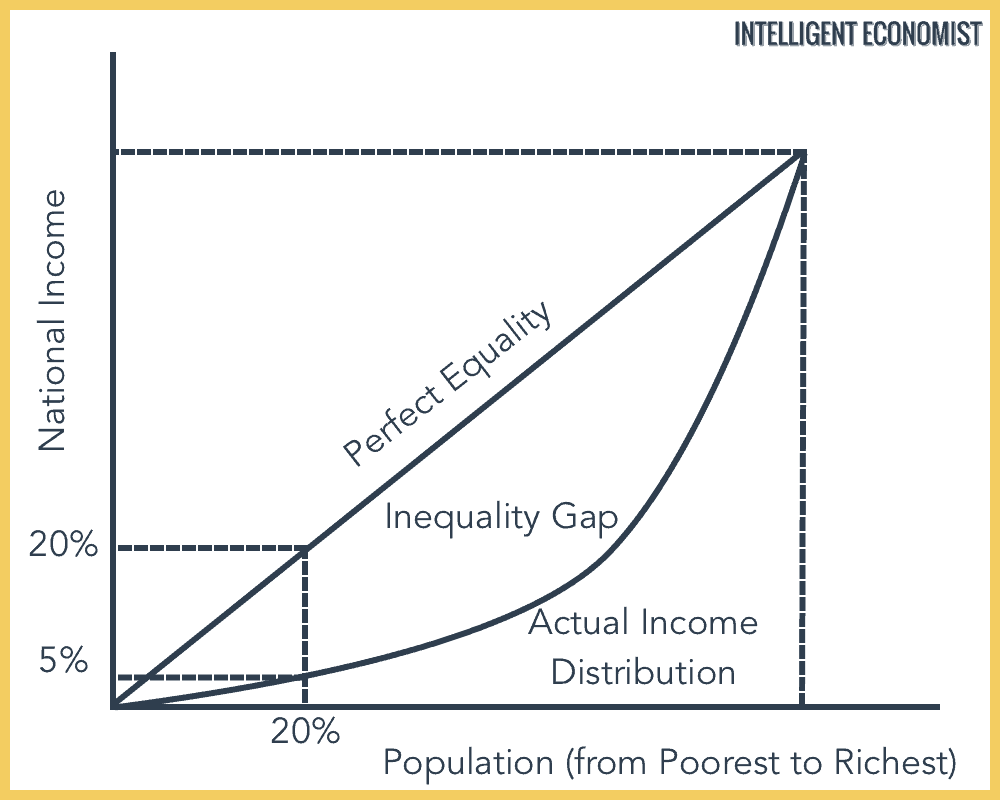
\includegraphics[width=0.5\textwidth]{03_Graphics/lorenz_curve}
\caption{Graph of Lorenz Curve \cite{CRYPTO:6}}
\end{center}
\end{figure}
A 45-degree line represents perfect wealth equality, so the Gini coefficient is essentially the ratio of the area that lies between the line of equality and the Lorenz curve. It is defined as one-half of the relative mean absolute difference: 
\begin{equation} 
G = \frac{\sum_{i=1}^{N}\sum_{j=1}^{N}\left | x_{i} - x_{j}\right |}{2 N^{2} \overline{x}} 
\end{equation}
where $x_{i}$ is the total wealth of person $i$ and $\overline{x}$ is the mean wealth across the population. Through the Gini coefficient, we can gain a significant understanding of the distribution of wealth as we simulate a Proof-of-Stake ecosystem.


% LMethods
%%% File encoding is ISO-8859-1 (also known as Latin-1)
%%% You can use special characters just like ä,ü and ñ

\chapter{Methods}

\section{Agent-based Modeling}
We used agent-based modeling in this project to simulate the effect of different Proof-of-Stake designs in economic centralization. Agent-based modeling simulates how micro-level decisions aggregate and interact to produce a macro-level system phenomena. For example, the micro pattern of the person-to-person spreading of the flu produces a macro pattern in the global landscape. In agent-based modeling, those micro-level interactions are encoded in the agents using simple rules to interact with each other. Instead of choosing completely random partners, agents usually only interact with those who are spatially close to them or connected to them on a social network. System level emergence, such as spread of disease, adoption of new technology, or composition of a community emerge as a result of such an interaction.

In our simulation, we designed the agent to be interacting as part of a network where they stake coins and get rewarded for becoming a validator. An agent's wealth, rules of interaction, and the selection process of validators between interacting agents are three elements that are particularly important in our model. Agents have heterogeneous internal states of wealth and greed preferences. Those internal states impact their interaction rules with other agents. While some rules are fixed for an agent's life, others rules can change in response to external environments, past interactions, expectations of future interactions, or even adopt a counterpart's strategy \cite{CRYPTO:9}. 

\section{Proof-of-Stake Simulation}
For us to begin agent-based modeling, we needed to define the network we want to simulate. Since we wanted an adequate sample size to simulate a network with a lot of activity, we configured the network to start with 10,000 nodes (or agents). We then defined a simulation around this network. We wanted to observe the effects of each Proof-of-Stake protocol on the network's Gini coefficient, so we defined two initial states for the network to begin in.

We wanted to observe what would happen to a network with a fairly even distribution, so our first initial state is normal distribution. In normal distribution, we distributed wealth across the network with a mean of 100 coins and a standard deviation of 10. This distribution with random numbers usually starts off with an initial Gini coefficient of 5\%. We also wanted to know the protocols' effects on an already wealth-centralized network like Bitcoin or Ethereum. Therefore, we have another initial state called "real" distribution. In this state, 80\% of the network starts off with just approximately 10 coins, another 15\% of the network starts off with about 100 coins, and the remaining 5\% start off with 1000 coins. This distribution starts off with a Gini coefficient of slightly below 80\%. We chose this distribution instead of replicating the current wealth distribution in Bitcoin because Bitcoin's wealth distribution was too extreme. We wanted to run simulations where it was still possible to observe a change in the Gini coefficient.

After initializing the nodes in the network, we repeatedly use a defined Proof-of-Stake protocol to determine the validator(s) of the next block and distribute the block reward. The base block reward for all simulations was set at 20 coins. In each Proof-of-Stake system we ran the simulation for 10,000 iterations and calculated the Gini coefficient to observe the long-term effects of each protocol.

Finally, in order to model network behavior, we decided to introduce elements of game theory into our design \cite{CRYPTO:3}. We designated a certain amount of "greed" for each node as a ratio from 0 to 1 where 0 is not at all greedy and 1 means completely greedy. This greed factor helps us determine node behavior as we progress through our simulation. In addition, the number of blocks mined and the node's greed ratio is also adjusted to match the distribution being used, with richer nodes beginning with a higher number of blocks mined and a higher greed ratio in a real distribution.

In our investigation, we evaluated the impact of reward distribution algorithms from different Proof-of-Stake systems (Pure Proof-of-Stake, Delegated Proof-of-Stake, and Extended Proof-of-Stake). We will also be applying principles of game theory in an attempt to design our own Proof of Stake protocol: Raffle Proof-of-Stake.

\subsection{Pure Proof-of-Stake}
Pure Proof-of-Stake (P-PoS) is one of the most straightforward approaches to modeling PoS systems. In P-PoS, players are pseudorandomly selected to propose blocks and vote on new blocks with their probability of selection being directly proportional to the amount of stake they have put into the system. The probability that a node $i$ is chosen as a validator is equal to the proportion of total wealth node $i$ holds, represented by the equation: 
\begin{equation}
P_i = \frac{i_{wealth}}{\sum_{n=1}^{N} n_{wealth}} 
\end{equation}
where N = number of nodes in the network. To model P-PoS, we first created a wealth distribution which takes the total amount of wealth in the network and calculates each user's proportional wealth relative to the total wealth amount. Using this probability distribution, we can then select a given number of validators from the network.

From the set of winners, the reward is evenly split from the prize pool by the number of total winners that were selected. Each winner then adds this reward to their personal wealth, and we recalculate the wealth distribution of the nodes before repeating the selection process.

The security of this system is based on the assumption that a majority of the verifiers are honest. Since the selection of block validators is conducted pseudorandomly, we assume that a majority of the network is honest to ensure that bad blocks are not validated. This system comes with some pros and cons based on this assumption. One benefit of this is that a small number of malicious users have a smaller percent chance of having a harmful influence on the network. This is because there is a small chance of these users being selected if they are a minority amount relative to the size of the network. In other PoS systems, it may be that a small set of users is in charge of selecting winners, which creates the risk of this small group being malicious. Pure Proof-of-Stake also assumes an honest majority because if a majority of stakers are acting maliciously, the value of the currency would ultimately decrease and those malicious users would also be losing money, which would disincentivize them from acting as so. A downside to this approach is that there is still a chance of malicious users being selected since the selection is entirely random. If a dishonest user were to obtain a large amount of stake, they could increase their chance of being selected and harm the network.

\subsection{Delegated Proof-of-Stake}
Delegated Proof-of-Stake is an abstraction on Proof-of-Stake where users stake to a pool rather than individually staking tokens to validate transactions and propose new blocks. Pools are then voted upon based on their stake value to then validate the transactions. This pool would then collect the block reward and distribute the winnings to its constituent stakers after keeping a cut. The reason behind using D-PoS instead of PoS is the benefits it has in terms of speed and scalability. There are many variations of D-PoS using different parameters, but in our simulations, the following D-PoS was used.

The ecosystem was set up with 10,000 participants. Network participants started with some random wealth which was generated based on a distribution. For our simulations we used both normal distributions, and real distributions in order to test the level of centralization in a network when it starts off balanced, and when it starts off already centralized. Following the initial deposit of wealth to each network participant, all network participants are considered to be pool operators. Every time-step, the participants decide which pool to allocate their stake toward.

\textbf{Decision criteria:}
\begin{itemize}
\item Number of blocks mined (proportional to number of blocks mined out of total)
\item Greed factor determines how much the miners take as a cut
\item Popularity regulates how likely stakers are to stake with the same pool again
\end{itemize}

For any delegate $d \in D$, where $D$ is the set of all delegates in the network, the probability mass function that any specific staker stakes with that specific delegate is represented by the following formula. 
\begin{equation}
p(d) = \frac{\mbox{numBlocksMined}(d) \times \mbox{popularity}(d)}{\sum_{i \in D} \mbox{numBlocksMined}(i) \times \mbox{popularity}(i)} 
\end{equation}
The popularity of a pool is determined by the following update formula where $n$ is a time step, $d \in D$ where $D$ is the set of all delegators, and $C$ is the set of all constituent nodes who delegated with delegator $d$ at time step $n$.
\begin{equation}
\mbox{popularity}(d)_{n+1} = \mbox{popularity}(d)_n * (0.995)^{\sum_{c \in C}1_{\{greed(d) > greed(c)\}}}
\end{equation}
Following the staking decisions, the D-PoS algorithm decides which pool to select as the next block creator\slash validator. It makes this decision through pseudorandom selection where the probability of being selected is proportional to that pool's percentage of total tokens staked. Once the block creator is chosen, the 20 coin block reward is distributed. The pool operator is able to decide how much of the reward they keep for themselves and how much gets distributed back to the constituents based on the greed factor. This process is then repeated with network participants giving tokens to a pool, a pool getting selected, and the rewards being distributed.

\subsection{Extended Proof-of-Stake}
The next type of Proof-of-Stake that we observed is Extended Proof-of-Stake (E-PoS). Although E-PoS has not been implemented in a real-world cryptocurrency, the concept was developed and we wanted to test it's proposed functionality \cite{CRYPTO:11}.

In E-PoS, the total transaction cost (sum of all transaction fees in a block) is recorded and maintained.
The first step in determining the validators for the designated blocks in E-PoS is to order all the blocks that need to be validated in decreasing order of transaction cost. Next, validators are given the option to place a bid for the block they want to mine. However, in order to become a potential candidate to validate a block, a node needs to have an account balance greater than the total transaction cost of the block. So, if a node does not contain enough funds, they cannot place a bid to potentially validate a block. After a certain amount of time, the network asks for a confirmation from each node that placed a bid for each block. The nodes first send a portion of their balance (equal to the transaction cost of the block) and some extra "commitment", which both get locked up. Commitment is the portion of the remaining balance of each node that is also sent with the transaction cost associated with being a potential candidate to validate a block. However, if no node contains a minimum amount of wealth that exceeds the total transaction cost of a block, the threshold for becoming a candidate for the block is reduced to allow the sender/receiver to validate the block themselves.

After all bids have been placed, the network runs an algorithm to determine which person to select as the validator for each block.
\spacing{1}
\begin{enumerate}
\item Find the node(s) who committed the most amount from their balance. For example, let's say that the total transaction cost of a block is 50 coins. Let's also assume that node A has 100 coins, while node B has 1000 coins each. Thus, each node is first required to commit 50 coins, leaving node A with 50 coins and node B with 950 coins. If node A then commits the remaining coins (50 coins), and node B commits (200 coins), node A will be chosen because node A committed 100\% of their remaining balance (50\slash50), while node B committed about 21\% (200\slash950). Thus, the node with the most commitment will be chosen.
\item Now, if two or more nodes commit the same amount of coins, then the network checks to see the amount of blocks each node has validated in the past (this would mean the network has to keep track of the number of blocks each node has validated). The network chooses the node that has validated the least amount of blocks. For example, if node A has 5 blocks validated and node B has 10 blocks validated, node A will be chosen.
\item Finally, if two or more nodes have mined the same number of blocks in the blockchain's history, then the node with the higher balance (more coins) is chosen to be the validator. So, from our first example, if node A had 100 coins and node B had 1000 (and we assume that they commit 100\% and both have 5 blocks validated), node B will be chosen since node B's account balance is greater.
\item If in the extreme case that two or more nodes have the exact same amount of coins, then one of those nodes is chosen at random.
\end{enumerate}
\onehalfspacing
However, there were some differences in our design as we could not implement all the features to their exact specifications. First, in the case when no one places a bid to validate a block, we first check to see if there is anyone that placed a bid for a block with a higher total transaction cost and run the selection algorithm on that list of nodes. Second, in the case when there are no alternatives to validate a block, a random node is chosen to become the validator. We implemented these two features because we focused on the selection process\slash incentive layer of a blockchain, so we did not keep track of the sender or receiver of a transaction.

\subsection{Our Own Design: Raffle Proof of Stake}
With the pros and cons of each of these PoS systems in mind, we decided to implement our own incentive layer based on a raffle system, named Raffle Proof-of-Stake (R-PoS). In our design, we used a game theoretic approach to enable nodes to become validators. Every staker can participate in a lottery to determine the next validator by offering up a fixed amount of their stake in exchange for raffle tickets. A node decides to participate in the raffle and pseudorandomly determines how many raffle tickets they wish to purchase weighted by their greed. The 'greedier' a node is, the more likely they are to purchase raffle tickets.

The coins used to purchase the tickets are then added to a "prize pool," in addition to the block reward. Once tickets are staked, a predetermined number of validators are chosen without replacement from the raffle pool. The validators then validate the block and are rewarded with a majority of the prize pool. The distribution ratio is represented by the equation: 
\begin{equation}
R_{winner} = \frac{v^2}{N}
\end{equation}
where $v$ is the number of validators and $N$ is the size of the network. With the remaining coins in the prize pool, another portion will be split out and evenly distributed among those who purchased raffle tickets as a consolation prize. The ratio of this split is determined by the number of people who participated in the raffle using the formula: 
\begin{equation}
R_{participant} = min\left (\frac{N_{participants}}{N_{nonparticipants}}, 0.9 \right )
\end{equation}
So, the more participants in the raffle, the higher the ratio of the consolation prize. Finally, the remaining balance of the prize pool is distributed evenly among the nodes who did not participate in the raffle and chose to receive some interest.

During this period, if a node won the raffle and earned money, their greed would increase by up to 10\%. If a node purchased tickets and won the raffle, but lost money overall, their greed will decrease by up to 30\%. If a node purchased tickets but did not win, they will increase or decrease their greed by a smaller amount (+\slash- 5\%) based on if the consolation prize covered or exceeded the cost of their tickets. The rest of the network who did not participate in the lottery will increase their greed by a miniscule amount (2\%) due to fear of missing out.

The motivation behind this design is that in other PoS protocols, the system incentivises hoarding of wealth. When this happens, it is very difficult for changes in wealth distribution to occur, and we end up seeing the rich becoming richer by holding onto their money. Our design incentivises spending, creating a micro-economy within the network with the raffle system. This allows the currency to shift around the nodes and hopefully establish a balance in wealth distribution. In this system, while it will be easier for the rich to win the raffle by purchasing many tickets, their opportunity cost increases with every ticket they buy. At a certain point, the raffle reward will not be able to cover the total cost of the raffle tickets purchased. Therefore, even if a node is rich, incentives pose an upper limit to the number of raffle tickets purchased and thereby limits their chance of winning. Moreover, our reward distribution method is done evenly, so the reward to a wealthy node will be the same as the reward to a node with a single coin.

Though this seems to cause participants to be disinterested in participating in the lottery, we expect the large prize pool for validators to incentivise participation. Moreover, the consolation prize for participating grows with more participants. So, many will choose to purchase just a single ticket hoping for a large participation rate to get the consolation prize, while other greedier nodes will aim for the much larger validation prize. Overall, there is a social optimum for more nodes to participate. We expect our addition of greedy behavior in the simulation model to be able to reflect these above behaviors, resulting in a more accurate modeling of our Proof-of-Stake design.


% Results
%%% File encoding is ISO-8859-1 (also known as Latin-1)
%%% You can use special characters just like �,� and �

\chapter{Results}
\begin{figure}[H]
\begin{center}
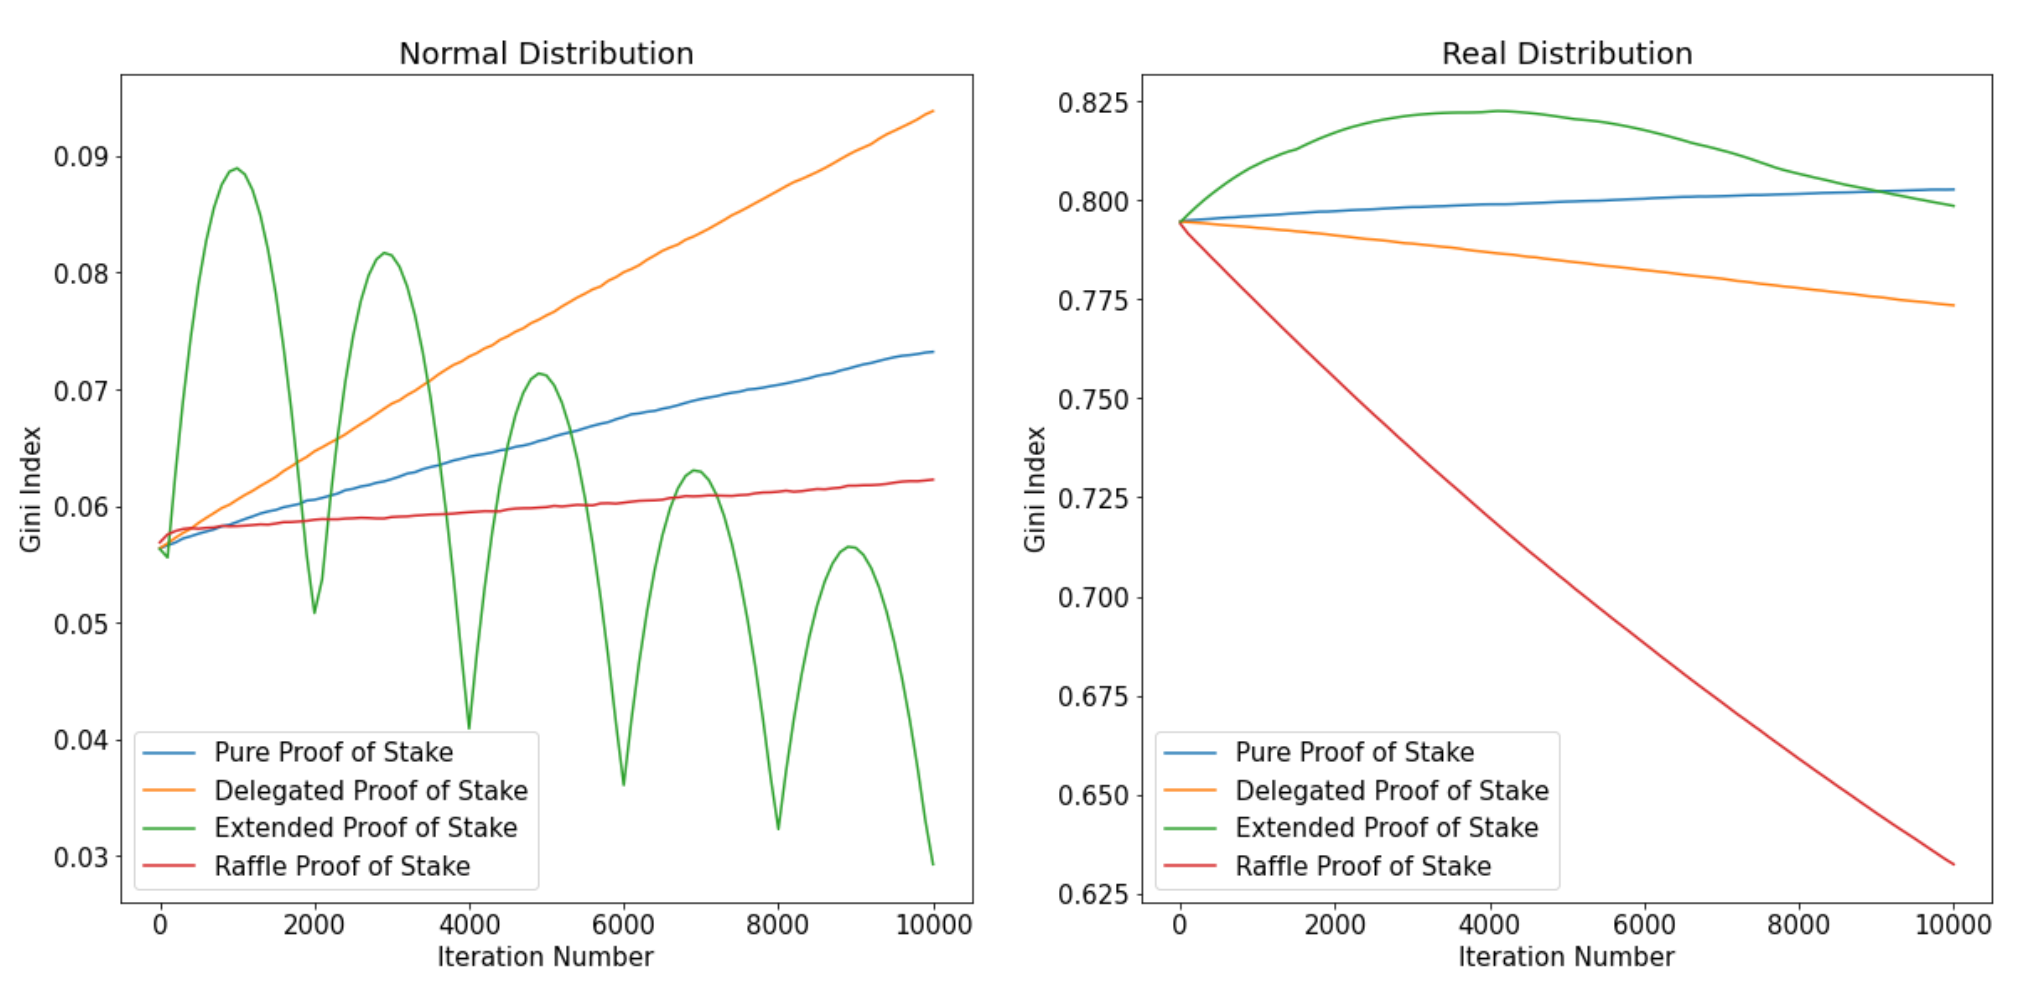
\includegraphics[width=1\textwidth]{03_Graphics/comparison}
\caption{Performance Comparison of All Protocols}
\label{fig:comp}
\end{center}
\end{figure}
\section{Pure Proof-of-Stake}
Based on our simulations with normal and real distributions of wealth, we found that P-PoS has a trend of increasing centralization over time. As described earlier, P-PoS carries out a pseudorandom selection process to determine validators of blocks, weighted by the amount of stake that the user has in the system. The more stake a user has, the more likely they are to be selected based on the factor of stake in random selection over time.
\begin{figure}[H]
\begin{center}
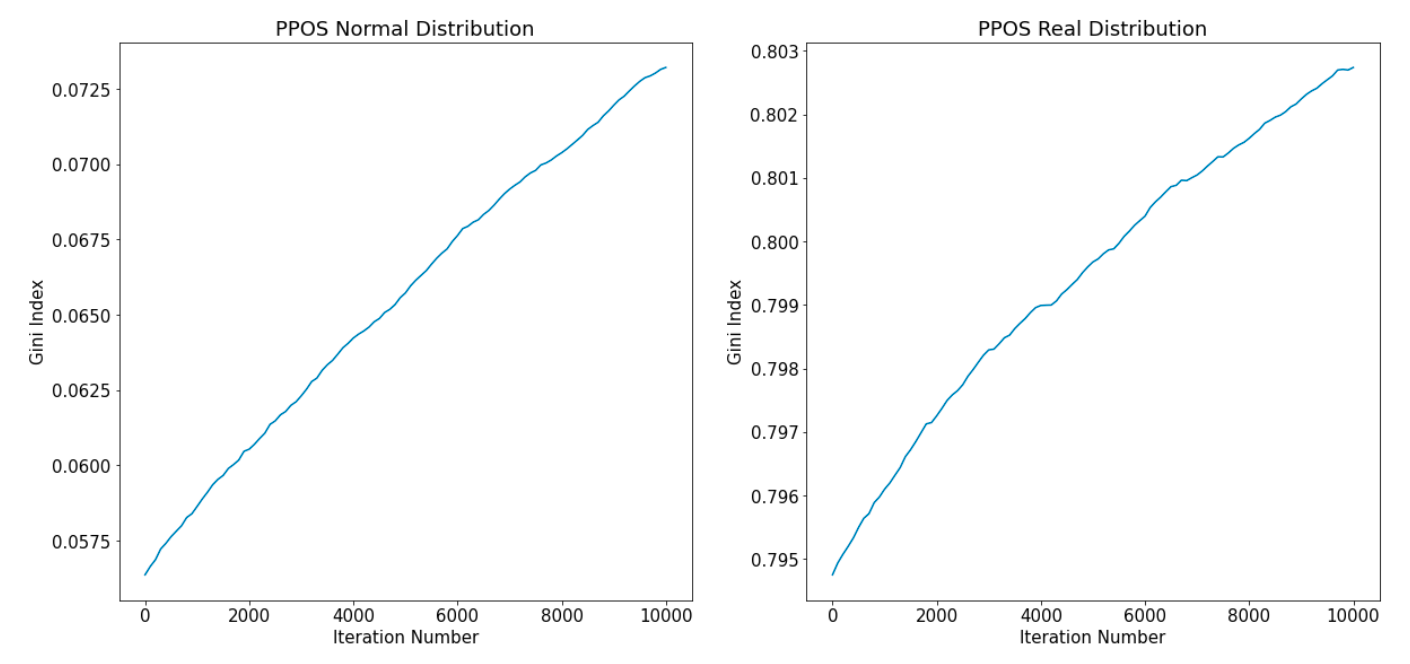
\includegraphics[width=1\textwidth]{03_Graphics/ppos_comp}
\caption{Performance of Pure Proof of Stake}
\end{center}
\end{figure}
Once a user is selected and wins the reward for verifying a block, they increase their total wealth and now have more that they can potentially stake in the system. This means as they keep winning, their probability of winning increases assuming they continue to increase the amount which they stake. In our model, we assume each user stakes their total wealth, as this presents the highest probability of them winning and there is no penalty for not being selected. As we can see in the performance graph of our model, the Gini coefficient increases linearly with the number of iterations of our simulation that are run.

\section{Delegated Proof-of-Stake}
\begin{figure}[H]
\begin{center}
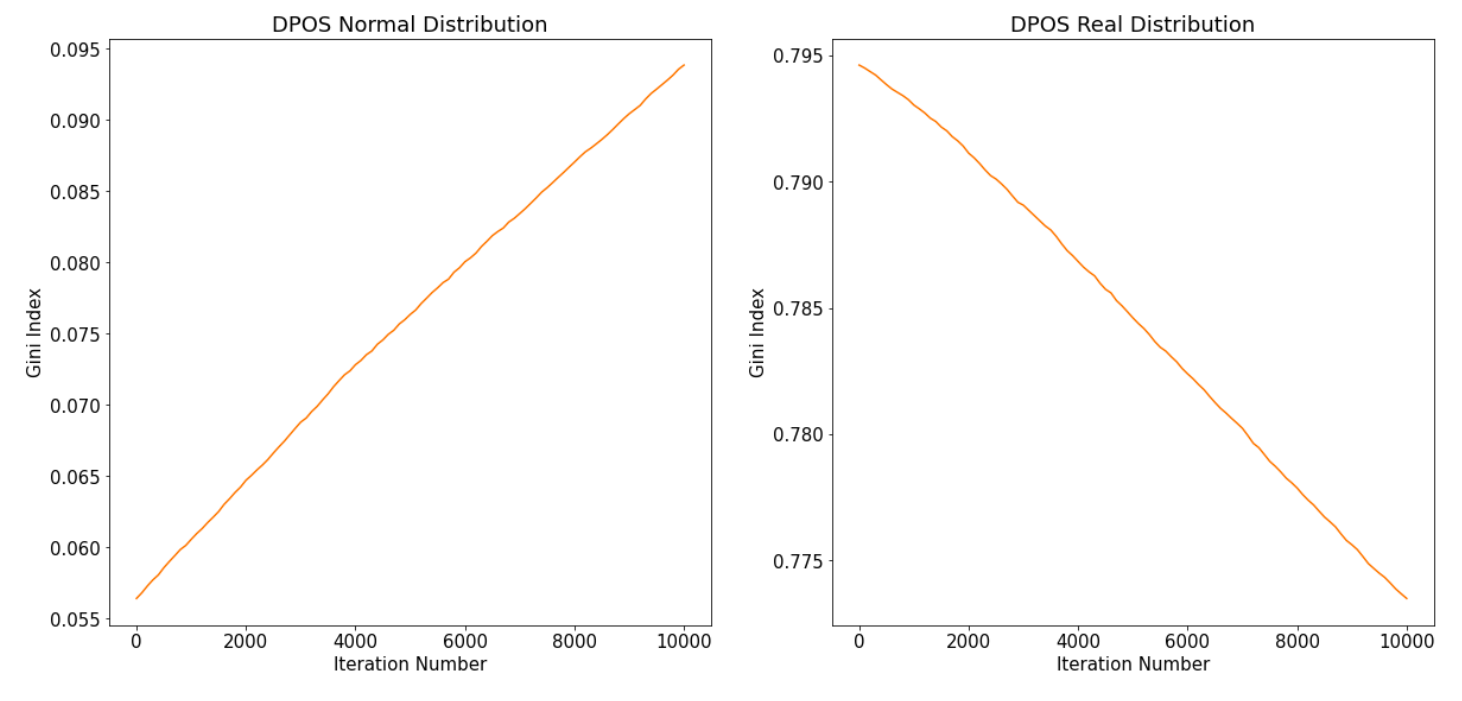
\includegraphics[width=1\textwidth]{03_Graphics/dpos_comp}
\caption{Performance of Delegated Proof of Stake}
\end{center}
\end{figure}
In a system that starts off very centralized, much like how a pre-mined coin, or a coin with reservations for early investors\slash developers, we see that delegated Proof-of-Stake performs fairly well in terms of reducing centralization. However, in a largely decentralized network, it causes rapid centralization of wealth.

The hypothesis for why the centralization shoots up rapidly in a very decentralized ecosystem is that the pool operators all rapidly increase their own wealth as they proceed to take a cut from every block mined. So their expected value from the network is higher since they are providing the service of creating and validating new blocks. However, in a highly centralized network, the trade-off between greed and popularity incentivizes the pools to compete and they end up splitting the wealth more fairly.

\section{Extended Proof-of-Stake}
For our simulation, we attempted to model this algorithm as closely as possible. To start off, we assigned each node an initial wealth and set the number of blocks validated of each node to 0. Afterwards, we created the blocks and assigned each block a random total transaction cost. After sorting the blocks in decreasing order of total transaction cost, we allowed each node to place a bid on the block they wanted to potentially validate. Assuming each node is greedy and wants to earn the most amount of coins, each node would place a bid on the highest total transaction cost block that does not exceed their total balance. In addition, the node would also commit 100\% of their remaining balance in an attempt to out-commit other nodes. We then place each node into a list of nodes associated with a given block. Finally, we run the E-PoS algorithm on each block, along with the corresponding list of potential nodes calculated from earlier.
\begin{figure}[H]
\begin{center}
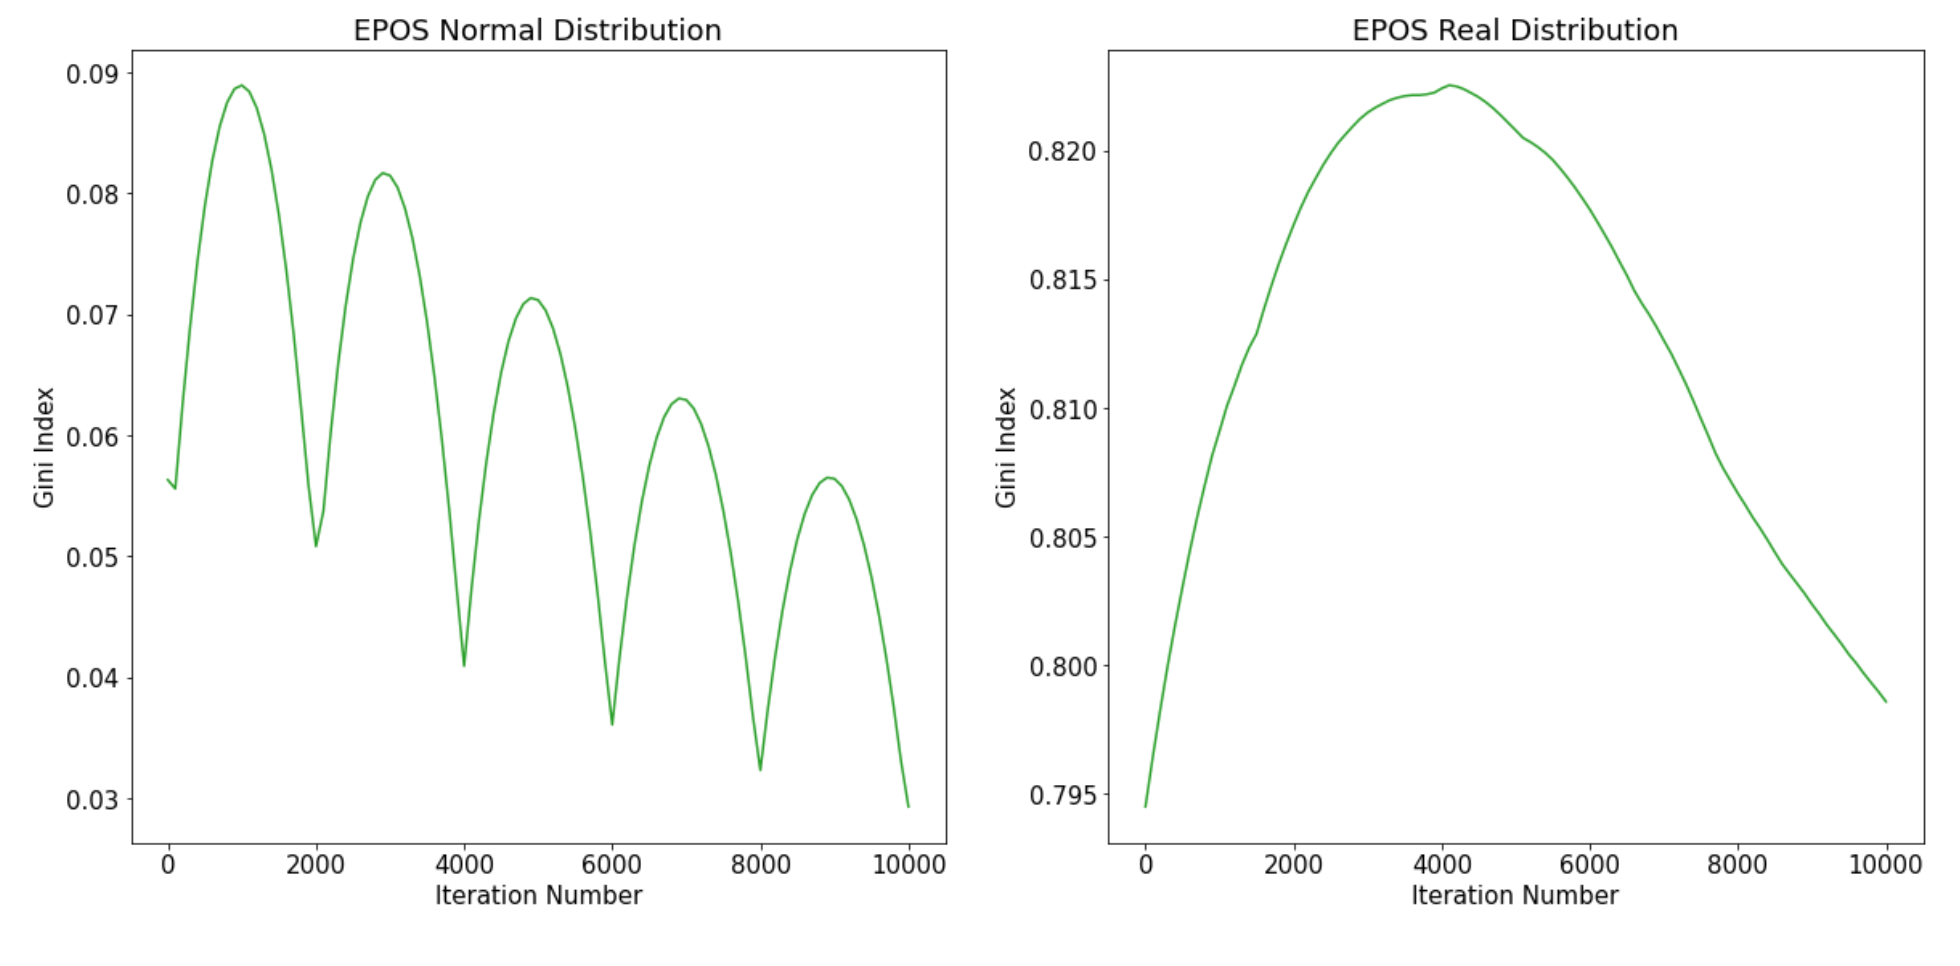
\includegraphics[width=1\textwidth]{03_Graphics/epos_comp}
\caption{Performance of Extended Proof of Stake}
\end{center}
\end{figure}
Based on the results of the simulation on normal distribution, we see that the graph consists of several bumps. This is because when people start off with approximately the same amount of wealth and 0 blocks validated, it basically becomes an in-order selection process. For example, if we start off with nodes A, B, and C (assuming similar wealth and 0 blocks validated), the first node chosen is the one with the most wealth, the next node chosen is the one with the second greatest wealth, and finally the node with the lowest wealth of the three nodes. Now that all nodes have 1 block validated, the same process will repeat.

For our testing purposes, we also ran a simulation on real distribution where the number of blocks validated for each node was proportional to their wealth. With these parameters, we noticed a different type of curve. When the wealth was more distributed (similar to a real distribution and assuming people with more wealth had more blocks validated), the Gini index decreased over time. This would indicate that E-PoS eventually reduces centralization over time due to the fact that the algorithm gives priority to people who validated less blocks. However, we cannot conclude that centralization will never increase again in the future.

\section{Raffle Proof of Stake}
\begin{figure}[H]
\begin{center}
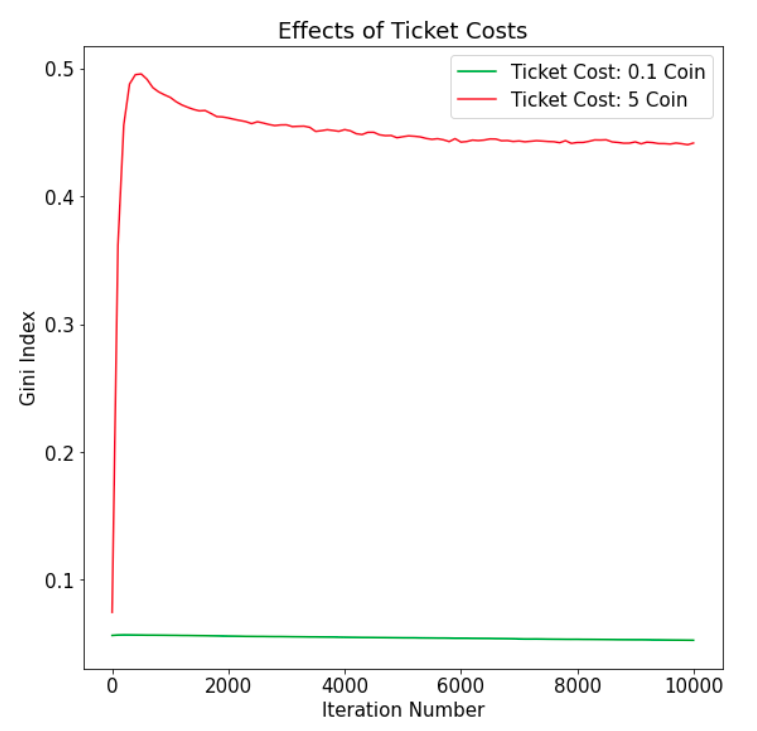
\includegraphics[width=0.5\textwidth]{03_Graphics/high_v_low}
\caption{Performance of Low vs. High Ticket Costs}
\end{center}
\end{figure}
Through the simulation of the Raffle Proof-of-Stake we designed, it was observed that in a network of 10,000 nodes beginning with a normal wealth distribution, the variable with the greatest impact on Gini coefficient was the participation cost or the cost per raffle ticket. With relatively lower ticket costs (i.e. 0.1 coin per ticket), the system performed very well with a miniscule change in Gini coefficient.

On the other hand, with high ticket costs (i.e. 5 coins per ticket), the system performed significantly worse, with the Gini coefficient rising at a much faster rate. Intuitively, this is due to the fact that increasing the ticket costs will also increase the size of the prize pool. This causes the shift in wealth to be in much larger increments after every raffle. Moreover, this theory is also supported by our findings during the investigation. We observed that with higher ticket costs, the average greed factor was higher than when the ticket costs were lower. This is because as the prize pool increased, so did the desire for nodes to participate. Therefore, an increase in ticket prices and the amount of participants caused the size of the prize pool to increase.

The same logic follows for low ticket costs. When ticket cost is 0.1 coin, the total prize pool decreases and the average node greed is also lower. We also realized that as more iterations passed, and new coins were mined, the reward from the raffle began to lose impact, and the effect on the Gini coefficient began to decrease. This is due to the average wealth of the network steadily increasing over iterations. So when the raffle ticket cost remained static, over time we observed the same effects as when ticket prices are very low. Therefore, we want to dynamically determine the cost of raffle tickets in accordance to the total wealth of the network.

By running the simulation multiple times with different pricing adjustments, we realized that the raffle Proof-of-Stake protocol works optimally when the average greed of the nodes remains at 0.5 (remember that greed is a ratio from 0 to 1). This means that when the network's greed is centered at the middle (or each node is "averagely" greedy), the distribution of wealth sets a good balance. With this implementation of raffle prizes, we then ran the simulations and compared them against the performances of the other Proof-of-Stake protocols we investigated. We observed that in terms of change in Gini coefficient, the raffle Proof-of-Stake performed the best.

From a network starting from a normal distribution of wealth, the increase in Gini coefficient was one one of the lowest compared to the other protocols (see Figure \textbf{\ref{fig:comp}}). In an already very centralized network, raffle Proof-of-Stake saw a very significant decrease in the Gini coefficient of the nodes. With these results, we can conclude that, on paper, raffle Proof-of-Stake outperforms all the other protocols we investigated in terms of reigning in the rate of increasing wealth centralization. In fact, if a network is already facing wealth centralization, the raffle Proof-of-Stake helps to mitigate it and redistribute the networks' wealth.


% Discussion
%%% File encoding is ISO-8859-1 (also known as Latin-1)
%%% You can use special characters just like �,� and �

\chapter{Discussion}

\section{Conclusion}
The purpose of this study was to evaluate centralization trends in various Proof-of-Stake models and determine whether or not centralization occurs in these systems overtime. By using agent based modeling techniques, we were able to simulate each system with a network of players and observe how each user's wealth changed over time. Based on our observation on the output of these models, we conclude that centralization does occur in Proof-of-Stake systems overtime. We also observe that our proposed model, Raffle Proof-of-Stake (R-PoS) can potentially decrease the rate of centralization, and in an ideal case, mitigate it as a major factor.

Looking at the combined results of the simulated network distribution, E-PoS starts off as the most centralized, but fluctuates down to have the lowest centralization coefficient as wealth becomes more distributed. P-PoS and D-PoS both show a linearly increasing trend of centralization overtime, with D-PoS having the fastest rate of increase. R-PoS has one of the lowest trends of centralization, though it is passed by the E-PoS model after around 8000 iterations. Overall, all of the defined models show a Gini Index greater than zero after starting from a baseline network.

In our simulation of a 'real' distribution, where 80\% of the network starts off with just approximately 10 coins, another 15\% of the network starts off with about 100 coins, and the remaining 5\% start off with 1000 coins, we observed slightly different characteristics of the models. All models start with a Gini Index around 0.80. We observed E-PoS having a logarithmic increase in centralization overtime and P-PoS slight increase. D-PoS begins to decrease slightly and our R-PoS system shows a strong linear decrease with more iterations.

\section{Limitations}
There were a few limitations our simulations faced. The first challenge was that we simulated the results of each of the various algorithms in isolated networks. In a real-world environment, there are thousands of different cryptocurrencies, each with their own network, and a node is free to convert their coins from one cryptocurrency to another. A node can then participate in the selection process within different networks, potentially making more money, and later  convert the coins back to the original cryptocurrency. The second limitation was that we focused on simulations on the incentive layer only. We did not analyze\slash model any other layers, so the results might be acceptable for the current layer, but they might negatively affect other layers. Thus, one layer might perform better within the simulations, but might hurt the overall blockchain overall if more layers were taken into account.

We also faced additional limitations within specific implementations. In D-PoS, our implementation allowed anyone to become a potential validator. However, in typical D-PoS, there are certain criteria a node must pass in order to become a delegate. This could impact centralization as it might eliminate many of the nodes in the network as potential delegates, thus leading to an increase in centralization over time.

In E-PoS, there were two main limitations we faced. The first limitation was determining who would validate a block if no one placed a bid for it. In the research paper, it mentioned that the total transaction cost of the block would decrease to enable the sender\slash receiver to validate it. Instead of this, we designed the system to select a node who placed a bid for a higher total transaction cost block. Additionally, in the case when there were no valid candidates (such as the first block), a random node was chosen from the network. The second limitation was determining the total transaction cost of the blocks. The initial E-PoS algorithm mentions that the number of potential validators should be roughly equal to the number of nodes in the network. This means that the total transaction cost should not exceed a majority of all the nodes' wealth and allow almost anyone to become a validator. However, since the main selection portion of the algorithm is to find validators with less blocks validated, this would introduce a potential sybil attack vulnerability as old validators can simply create new accounts (thus appearing to have 0 blocks validated) and have a better chance of being selected as a validator.

For R-PoS, it is extremely difficult to model human risk tolerance. We used a model that assumes that people will become greedier the more they keep winning and less greedy when they keep losing. However, this does not mean that someone on either end will continue to remain on the same decision pattern. It was even more difficult predicting a node's risk level when they laid in the middle of the greed spectrum because the issue was not only whether they stake or not, but also how many raffle tickets they would choose to buy.

\section{Future Work}
Overall, this process of creating simulations led to a whole new series of questions that could be answered with more work. The first thing that we would note in our simulations is that all of the networks exist in isolation. In the real world, network participants in one network have the ability to sell their tokens (and possibly incur some fee), and then allocate their resources to another token. In this regard, there may be some interactions between different tokens that we have not explored. If we had more time we would have been able to test integrating various combinations of Proof of Stake systems.

There was also some experimentation that we could have done with the simulation parameters. We had a fixed 10,000 participants in each simulation. We could have seen the results as the number of participants changes over time. We also have the additional complexity of non-staking transactions that wasn't completely encoded in the simulations. We assumed that there were some random variables representing the transaction fees, but we didn't model the transfer of wealth aside from the staking rewards. In doing so, we may find different results if the model ends up self re-balancing. We would also like to research further into different initializations of wealth distribution and block rewards.

On top of the future work regarding the overall simulation, there are some things that each individual model could also have explored. On the P-POS front, we decided that our algorithm will select 5 validators, which assumes only 5 blocks needed to be validated each round. However, maybe if there are more\slash less blocks, the number of validators would change and centralization may be impacted. For D-POS, we have constructed the simulation such that all network participants could be mining pool operators. This however is infeasible in practice because of the effort, technical skill, and resources needed to host a full validator. Thus, it would have been better to model the network with these costs accounted for. For the R-PoS and D-POS models we also could have implemented a bit more formal Nash equilibrium game theoretic decisions based on discounted future rewards that may have led to different playing strategies.
Overall, this research has opened up the possibility of exploring many aspects of Proof-of-Stake and the role it plays on centralization.


% References
\nocite{*}
\bibliographystyle{ieeetr}
\bibliography{02_Chapters/References}


\end{document}
% ------------------------------------------------------------------
%
% #######################
% End: Document
% #######################
